\documentclass[]{book}
\usepackage{lmodern}
\usepackage{amssymb,amsmath}
\usepackage{ifxetex,ifluatex}
\usepackage{fixltx2e} % provides \textsubscript
\ifnum 0\ifxetex 1\fi\ifluatex 1\fi=0 % if pdftex
  \usepackage[T1]{fontenc}
  \usepackage[utf8]{inputenc}
\else % if luatex or xelatex
  \ifxetex
    \usepackage{mathspec}
  \else
    \usepackage{fontspec}
  \fi
  \defaultfontfeatures{Ligatures=TeX,Scale=MatchLowercase}
\fi
% use upquote if available, for straight quotes in verbatim environments
\IfFileExists{upquote.sty}{\usepackage{upquote}}{}
% use microtype if available
\IfFileExists{microtype.sty}{%
\usepackage{microtype}
\UseMicrotypeSet[protrusion]{basicmath} % disable protrusion for tt fonts
}{}
\usepackage[margin=1in]{geometry}
\usepackage{hyperref}
\hypersetup{unicode=true,
            pdftitle={Ciencia de Datos para Gente Sociable},
            pdfauthor={Antonio Vazquez Brust},
            pdfborder={0 0 0},
            breaklinks=true}
\urlstyle{same}  % don't use monospace font for urls
\usepackage{natbib}
\bibliographystyle{apalike}
\usepackage{longtable,booktabs}
\usepackage{graphicx,grffile}
\makeatletter
\def\maxwidth{\ifdim\Gin@nat@width>\linewidth\linewidth\else\Gin@nat@width\fi}
\def\maxheight{\ifdim\Gin@nat@height>\textheight\textheight\else\Gin@nat@height\fi}
\makeatother
% Scale images if necessary, so that they will not overflow the page
% margins by default, and it is still possible to overwrite the defaults
% using explicit options in \includegraphics[width, height, ...]{}
\setkeys{Gin}{width=\maxwidth,height=\maxheight,keepaspectratio}
\IfFileExists{parskip.sty}{%
\usepackage{parskip}
}{% else
\setlength{\parindent}{0pt}
\setlength{\parskip}{6pt plus 2pt minus 1pt}
}
\setlength{\emergencystretch}{3em}  % prevent overfull lines
\providecommand{\tightlist}{%
  \setlength{\itemsep}{0pt}\setlength{\parskip}{0pt}}
\setcounter{secnumdepth}{5}
% Redefines (sub)paragraphs to behave more like sections
\ifx\paragraph\undefined\else
\let\oldparagraph\paragraph
\renewcommand{\paragraph}[1]{\oldparagraph{#1}\mbox{}}
\fi
\ifx\subparagraph\undefined\else
\let\oldsubparagraph\subparagraph
\renewcommand{\subparagraph}[1]{\oldsubparagraph{#1}\mbox{}}
\fi

%%% Use protect on footnotes to avoid problems with footnotes in titles
\let\rmarkdownfootnote\footnote%
\def\footnote{\protect\rmarkdownfootnote}

%%% Change title format to be more compact
\usepackage{titling}

% Create subtitle command for use in maketitle
\newcommand{\subtitle}[1]{
  \posttitle{
    \begin{center}\large#1\end{center}
    }
}

\setlength{\droptitle}{-2em}
  \title{Ciencia de Datos para Gente Sociable}
  \pretitle{\vspace{\droptitle}\centering\huge}
  \posttitle{\par}
\subtitle{Una introducción a la exploración, análisis y visualización de datos}
  \author{Antonio Vazquez Brust}
  \preauthor{\centering\large\emph}
  \postauthor{\par}
  \predate{\centering\large\emph}
  \postdate{\par}
  \date{2018-07-30}

\usepackage{booktabs}

\begin{document}
\maketitle

{
\setcounter{tocdepth}{1}
\tableofcontents
}
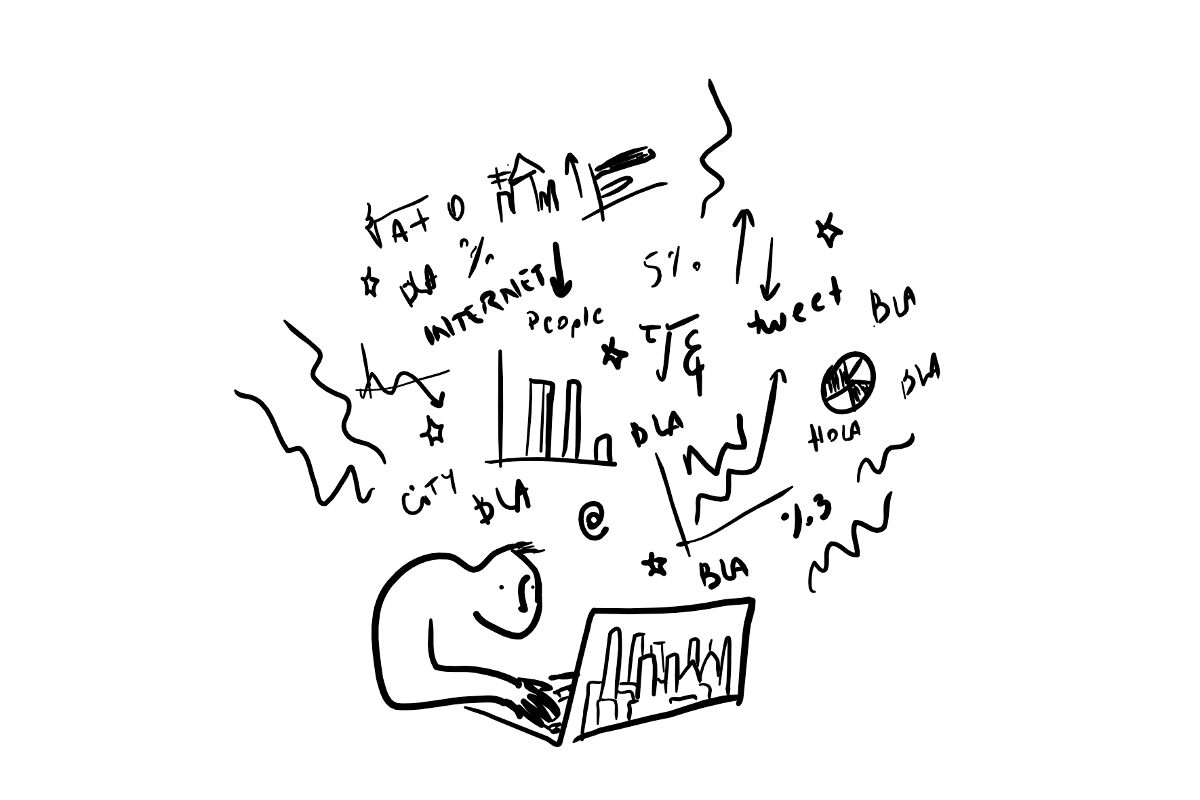
\includegraphics[width=16.67in]{imagenes/portada}

\chapter*{¿Para quién es esto?}\label{para-quien-es-esto}
\addcontentsline{toc}{chapter}{¿Para quién es esto?}

Este libro fue escrito con una audiencia en mente formada por
urbanistas, sociólogos, politólogas y otros entusiastas que se acercan
al tema desde las Ciencias Sociales. Aún así, y por supuesto, todas las
personas y algoritmos con capacidad de procesar lenguaje son
bienvenidas.

Espero que el tono introductorio del texto, así como el esfuerzo puesto
en explicar los conceptos con la mayor simplicidad posible, resulten de
interés para un público amplio.

No hace falta ningún conocimiento previo de programación; todas las
herramientas necesarias serán explicadas sobre la marcha.

\chapter*{Antes de empezar}\label{antes-de-empezar}
\addcontentsline{toc}{chapter}{Antes de empezar}

Para practicar los ejemplos que se explicarán a lo argo del libro, es
necesario instalar el \href{https://cloud.r-project.org/}{lenguaje de
programación R}, y la interfaz gráfica
\href{https://www.rstudio.com/products/rstudio/download/}{RStudio
Desktop}.

\chapter{¿Qué es la ciencia de datos?}\label{que-es-la-ciencia-de-datos}

Placeholder

\section{¿Qué significa hacer ciencia de
datos?}\label{que-significa-hacer-ciencia-de-datos}

\chapter{Una presentación a toda marcha de
R}\label{una-presentacion-a-toda-marcha-de-r}

Placeholder

\section{Nuestro primer proyecto en
R}\label{nuestro-primer-proyecto-en-r}

\subsection{A investigar: ¿Cual es la diferencia en mortalidad infantil
entre el sur y el norte de la Ciudad Autónoma de Buenos
Aires?}\label{a-investigar-cual-es-la-diferencia-en-mortalidad-infantil-entre-el-sur-y-el-norte-de-la-ciudad-autonoma-de-buenos-aires}

\subsection{Crear un proyecto en
RStudio}\label{crear-un-proyecto-en-rstudio}

\subsection{Escribiendo un script}\label{escribiendo-un-script}

\subsection{Cargar los datos}\label{cargar-los-datos}

\section{Visualización: la exploración gráfica de la
información}\label{visualizacion-la-exploracion-grafica-de-la-informacion}

\subsection{Haciendo mapas}\label{haciendo-mapas}

\subsection{Agregando datos}\label{agregando-datos}

\section{El veredicto final}\label{el-veredicto-final}

\subsection{¿Cuál es la diferencia en mortalidad infantil entre el sur y
el norte de la Ciudad Autónoma de Buenos
Aires?}\label{cual-es-la-diferencia-en-mortalidad-infantil-entre-el-sur-y-el-norte-de-la-ciudad-autonoma-de-buenos-aires}

\chapter{Poniendo los datos en forma}\label{poniendo-los-datos-en-forma}

Placeholder

\section{Primeros pasos al examinar un conjunto de datos
nuevo}\label{primeros-pasos-al-examinar-un-conjunto-de-datos-nuevo}

\section{\texorpdfstring{Cruzando variables: la operación
\texttt{join}}{Cruzando variables: la operación join}}\label{cruzando-variables-la-operacion-join}

\section{Transformando los datos}\label{transformando-los-datos}

\subsection{\texorpdfstring{Seleccionar columnas con
\texttt{select()}}{Seleccionar columnas con select()}}\label{seleccionar-columnas-con-select}

\subsection{\texorpdfstring{Filtrar filas con
\texttt{filter()}}{Filtrar filas con filter()}}\label{filtrar-filas-con-filter}

\subsubsection{Comparaciones}\label{comparaciones}

\subsubsection{Operadores lógicos}\label{operadores-logicos}

\subsection{\texorpdfstring{Ordenar filas con
\texttt{arrange()}}{Ordenar filas con arrange()}}\label{ordenar-filas-con-arrange}

\subsubsection{Valores faltantes}\label{valores-faltantes}

\subsection{\texorpdfstring{Agregar nuevas variables con
\texttt{mutate()}}{Agregar nuevas variables con mutate()}}\label{agregar-nuevas-variables-con-mutate}

\subsection{\texorpdfstring{Extraer sumarios con
\texttt{summarise()}}{Extraer sumarios con summarise()}}\label{extraer-sumarios-con-summarise}

\subsection{\texorpdfstring{¡BONUS! El operador ``pipe'':
\texttt{\%\textgreater{}\%}}{¡BONUS! El operador pipe: \%\textgreater{}\%}}\label{bonus-el-operador-pipe}

\chapter{Visualización}\label{visualizacion}

Placeholder

\section{\texorpdfstring{Una buena visualización para empezar: el
\emph{scatterplot}}{Una buena visualización para empezar: el scatterplot}}\label{una-buena-visualizacion-para-empezar-el-scatterplot}

\section{Ajustando color y tamaño}\label{ajustando-color-y-tamano}

\section{Facetado}\label{facetado}

\section{Gráficos de barras}\label{graficos-de-barras}

\section{Histogramas}\label{histogramas}

\section{Preparando una visualización para
compartir}\label{preparando-una-visualizacion-para-compartir}

\section{Otras visualizaciones}\label{otras-visualizaciones}

\chapter{Modelado estadístico}\label{modelado-estadistico}

Placeholder

\section{Regresión lineal simple}\label{regresion-lineal-simple}

\subsection{Regresión con una variable
numérica}\label{regresion-con-una-variable-numerica}

\subsection{Revolviendo los residuos}\label{revolviendo-los-residuos}

\subsection{Regresión con una variable
categórica}\label{regresion-con-una-variable-categorica}

\section{Regresión con múltiples
variables}\label{regresion-con-multiples-variables}

\chapter{Información geográfica y
mapas}\label{informacion-geografica-y-mapas}

Placeholder

\section{Los datos georreferenciados}\label{los-datos-georreferenciados}

\section{Formatos de archivo}\label{formatos-de-archivo}

\section{Explorando un archivo con información
geográfica}\label{explorando-un-archivo-con-informacion-geografica}

\section{Visualizando información
geográfica}\label{visualizando-informacion-geografica}

\section{Volcando en el mapa información de múltiples
fuentes}\label{volcando-en-el-mapa-informacion-de-multiples-fuentes}

\section{Combinando capas
geográficas}\label{combinando-capas-geograficas}

\bibliography{book.bib,packages.bib}


\end{document}
